\section{Eredmények}
\subsection{Szilárd kontaktusú mikroelektródok használata mérőcsúcsként}
A hagyományos, folyadékkontaktusú elektródokhoz képest a minden más területen megegyező szilárd kontaktusú elektródok ellenállása kisebb.
Ennek két oka van.
A szilárd kontaktus letolható egészen a pipetta csúcsáig, csökkentve ezzel a nagy ellenállású ion-szelektív membrán vastagságát.
A másik oka az, hogy a belső oldat helyett -- melynek nagy ellenállása van --, egy módosított szénszál -- melynek kis ellenállása -- nyújtja az ion-elektron interfészt.
Ha $R$ kisebb, $RC$ is kisebb, és a potenciometriás cella gyorsabb.

Készítettem két Mg$^{2+}$ ion-szelektív elektródot; egy folyadék- és egy szilárd-kon\-tak\-tu\-sút.
Ezen különbségen kívül azonos módon készítettem őket.
Elvégeztem az alapvető jellemzésüket.
A válasz karakterisztikájukat az $R$ és a 95\% válaszidő mérésével ($\tau_{95}$) vizsgáltam.
A feszültségosztó módszer során mért értékekből a folyadék- és szilárd-kontaktusú elektródok ellenállása $4.8~$G$\ohm$ és $0.56~$G$\ohm$ volt.
Ezen értékek alapján a szilárd-kontaktusú változat használatakor kisebb torzítású képek várhatóak ugyanolyan pásztázási paraméterek használata esetén.

Ennek igazolására pásztázásokat végeztem mindkét elektróddal egy Mg$^{2+}$ ion forrás felett, melyet egy mikropipetta szolgáltatott.
A mikropipettában 0.1 M MgCl$_2$ oldat volt.
A \ref{fig:solid_liquid_pipette}. ábra mutatja az eredményeket a (A) folyadék- és a (B) szilárd-kontaktusú mikroelektród használata esetén.
Mindkét kép ugyanazzal a sebességgel lett rögzítve.
Könnyen észrevehető az folyadék-kontaktusú mikroelektród használata során tapasztalható X irányú torzítás, ami várható is volt a nagy ellenállása alapján.
Ugyan megfigyelhető a torzítás a másik képen is, de ennek mértéke sokkal kisebb.
Fontos különbség továbbá, hogy a legnagyobb észlelt magnézium-ion koncentrációk eltérőek.
A szilárd-kontaktusú elektród esetén ez az érték $10^{-2.5}$ M, míg a folyadék-kontaktusú elektród esetén csak $10^{-3.4}$ M.
Ennek valószínű oka az, hogy a folyadék-kontaktusú mikroelektródokt alkalmazó cella nem bír lépést tartani a magnézium ion koncentrációjának változásával.

\begin{figure}
\centering
% trim = top left bottom right
\includegraphics[trim = 10mm 30mm 0mm 10mm, clip, width=0.35\textwidth, angle=-90]{img/mg_pipette/liquid_Mg.eps} \includegraphics[trim = 10mm 30mm 0mm 10mm, clip, width=0.35\textwidth, angle=-90]{img/mg_pipette/solid_Mg.eps}
\caption{PEKM képek a Mg$^{2+}$ ion forrás felett 100 $\upmu$m magasságban.
(A) folyadék-, and (B) szilárd-kontaktusú mikroelektród használata esetén.
Pásztázási sebesség mindkét esetben: 12.5 $\upmu$m/s.}
\label{fig:solid_liquid_pipette}
\end{figure}

A szilárd-kontaktusú elektródok alkalmazásának egy példáját is bemutattam disszertációmban; magnézium és ötvözeteinek galvanikus korróziójának vizsgálata PEKM technikával.
AZ63 magnézium-alumínium ötvözet felett térképeztem a magnézium ion koncentrációjának tér- és időbeli változását.
Vertikális Mg$^{2+}$ ion profilokat rögzítettem különböző időpontokban indítva a mérést, az AZ63 és vas minták galvanikus korróziója során.
Ezen profilokat felhasználva a Mg$^{2+}$ fluxus a felületen keresztül megbecsülhető:

\begin{equation}
\label{eq:corrosion_current}
        \Omega = 4 D C_s a
\end{equation}
ahol $\Omega$ az AZ63 minta felületén keresztüli Mg$^{2+}$ fluxus, $D$ a Mg$^{2+}$ diffúzióállandója, $C_s$ a Mg$^{2+}$ közvetlenül a felület mellett észlelhető koncentrációja ($z$ = 0 $\upmu$m magasságban), $a$ a minta sugara.
Mint egyetlen ismeretlen, $\Omega$ kiszámítható.

A galvánpár közötti korróziós áramot megmértem egy másik módszerrel.
Faraday törvényét használva kiszámoltam a korróziós áramot az előző módszer alapján is.
Jó egyezést kaptam a két módszer használata esetén.

\subsection{Pásztázási algoritmusok optimalizálása}
A második és harmadik megközelítés során a potenciometriás válaszfüggvény tulajdonságait használom fel:

\begin{equation}
\label{eq:rc}
        E_{cell}(t_{e}) = E_{cell}(\infty) + [E_{cell}(0) - E_{cell}(\infty)]e^{-t_{e}/RC}
\end{equation}
ahol $E_{cell}(t)$ és $E_{cell}(\infty)$ a potenciál különbség $t_{e}$ és ,,végtelen'' idő elteltével, $E_{cell}(0)$ a kezdeti potenciál különbség.
Minél különbözőbb $E_{cell}(0)$ és $E_{cell}(\infty)$, annál nagyobb lesz a különbség $E_{cell}(\infty)$ és $E_{cell}(t_{e})$ között.
Egy kép torzítása a $E_{cell}(\infty)$ és $E_{cell}(t_{e})$ közti különbségek átlagaként fogható fel.
Ez csökkenthető a pásztázási mintázatok és algoritmusok körültekintő optimalizálásával úgy, hogy a mérőcsúcs a lehető legkevesebbszer halad át olyan pontok között, ahol nagy a különbség $E_{cell}(0)$ és $E_{cell}(\infty)$ között.

Az eredményeket a \ref{fig:simulations}. ábra mutatja, mely igazolta a feltételezéseket; optimalizált algoritmusok használatakor kisebb torzítású képek nyerhetők.
Az eredményeket szimulációkkal is alátámasztottam, melyek a disszertációmban megtalálhatók.

\begin{figure}
\centering
% trim = top left bottom right
\includegraphics[trim = 10mm 30mm 0mm 10mm, clip, width=0.35\textwidth, angle=-90]{img/polar/meander.eps} \includegraphics[trim = 10mm 30mm 0mm 10mm, clip, width=0.35\textwidth, angle=-90]{img/polar/arc.eps}
\caption{PEKM képek 100 $\upmu$m magasságban egy korong alakú forrás felett, (A) meander és (B) körívmenti pásztázás eseténs.
Az indikátor elektród egy pH-érzékeny antimon mikroelektród volt.}
\label{fig:simulations}
\end{figure}

\subsection{Potenciometriás PEKM képek dekonvolúciója}
A harmadik módszer amit kidolgoztam a potenciometriás válaszfüggvény (\ref{eq:rc}. egyenlet) inverzét használja dekonvolúciós függvényként.
A $t_e$, $E_{cell}(0)$, $E_{cell}(t_e)$ és $E_{cell}(\infty)$ közötti összefüggés jól ismert, $E_{cell}(\infty)$ értéke megjósolható minden egyes pontra.

\begin{figure}
\centering
% trim = top left bottom right
\includegraphics[trim = 10mm 30mm 0mm 10mm, clip, width=0.35\textwidth, angle=-90]{img/pH_2D_Sb/13121313.eps}\includegraphics[trim = 10mm 30mm 0mm 10mm, clip, width=0.35\textwidth, angle=-90]{img/pH_2D_Sb/13121313_deconvoluted.eps}%\includegraphics[trim = 20mm 30mm 0mm 20mm, clip, width=0.3\textwidth, angle=-90]{13121313_diff.eps}
\caption{PEKM pH kép dekonvolúció (A) előtt és (B) után.
Indikátor elektród: antimon pH-érzékeny mikroelektród.
A potenciál skálák különbözőek a képen.
A dekonvolúció nem csak a vizsgált céltárgy alakját állítja helyre a képen, hanem a mért maximális érték nagyságát is.
A raszter pásztázási mintázatot használtam a meander algoritmussal, a kép bal alsó sarkából indulva.}
\label{fig:deconvolution}
\end{figure}

Két dimenziós PEKM pásztázásokat végeztem körszimmetrikus grafit anód felett (\ref{fig:deconvolution}A ábra) a meander algoritmussal.
A meander algoritmus pásztázási vonalainak mentén a torzítás jól észrevehető.
A kép dekonvolúciójával a várt, körszimmetrikus kép nyerhető (\ref{fig:deconvolution}B ábra).
A körszimmetria megjelenése mellett a maximális mért potenciál érték is változott.
A maximális érték az eredeti képen $-300$ mV, a dekonvolúció után pedig $-260$ mV.
A dekonvolúció jóságát sokkal lassabb vonalpásztázásokkal igazoltam, ahol nem lépett fel torzítás.

Hasonló eredményeket kaptam ionofór alapú ion-szelektív mikropipetták alkalmazása során.
Az eredmények megtalálhatók a disszertációmban, itt hely hiány miatt nem mutatom be őket.

A technika alkalmazhatóságának bemutatásaként szénacél minta korrózióját vizsgáltam.
A rögzített kép a várakozásoknak megfelelően torzított lett.
A minta szabálytalan alakja nem látszott az eredeti képen.
Dekonvolúció után jó egyezést kaptam az optikai képhez képest.
Mint korábban, a különbség az eredeti és a feldolgozott kép között nagy.
Az eredeti kép alapján a minta feletti pH változást alulbecsültem volna 1 egységgel.
Más konklúzió vonható le a nyers és a feldolgozott kép alapján.

Egy másik technika amit kipróbáltam az úgynevezett ,,vak dekonvolúció''.
Dekonvolúció lehetséges akkor is, ha nem ismert a függvény összes paramétere.
Egy korábbi PEKM képet dolgoztam fel különböző időállandókat, köztük a helyes, mért értlket is  használva. 
A legjobb eredményt természetesen akkor kaptam, mikor a mért időállandót használtam dekonvolúciós paraméterként.
Ami érdekes a technikában, hogy a helyes érték ránézésre is megállapítható, mert a meander vonal menti torzítás jól észrevehető.
A technika egy továbbfejlesztett változata statisztikai megközelítés lenne.
A feldolgozott képek közül elméletileg az a legkisebb torzítású, amelyik a legkisebb korrelációt mutat a használt pásztázási algoritmussal.

\subsection{Az elektromos tér hatása potenciometriás PEKM képalkotásra}
Galvanikus korrózió során ionok oldódnak ki az anód felületéről.
Az indikátor elektród potenciálja főleg az elsődleges ion aktivitásától függ.
Ha azonban jelen van egy elektromos mező is a vizsgált rendszerben, ennek a mérőcsúcsnál mutatkozó értéke egyszerűen hozzáadódik a mért értékhez:

\begin{equation}
\Delta E=E_M-E_R + (\phi_M - \phi_R)
\label{eq:potential}
\end{equation}
ahol $\Delta E$ a mért potenciál különbség, $E_M$ és $E_R$ az indikátor és a referencia elektródok potenciálja, $\phi_M$ és $\phi_R$ az elektromos mező helyi potenciáljai az indikátor, és a referencia elektród helyénél.
Az elektromos mezőt galvanikus korrózió során a galvánpár felületei között fellépő potenciál különbség okozza.

Számos cikk számol be ellentmondásos eredményekről, melyeket olyan rendszerekben mértek, ahol erős elektromos mező volt jelen.
Az ellentmondás megmagyarázható az elektromos mező a mért potenciálhoz való direkt hozzájárulásával.

\begin{figure}
\centering
\begin{tikzpicture}
\begin{axis}[ymin=-75, ymax=200, xmin=0, xmax=680, xlabel={idő, s}, ylabel={E, mV vs Ag/AgCl/ 3M KCl}, clip marker paths=true, width=7cm, height=7cm, legend style={draw=none}, legend cell align=left]
\addplot [domain=-30:100, color=red, mark=*] table {data/field/on_off_100.txt};
\addplot [domain=-30:100, color=blue, mark=*] table {data/field/on_off_1000.txt};
%\node[anchor=north east] at (rel axis cs:0.98,0.98) {B};
\node[red, above right] at (axis cs:10,20) {h = 100 $\upmu$m};
\node[blue, above right] at (axis cs:10,-50) {h = 1000 $\upmu$m};
\draw [black, ->] (axis cs:320,125) -- (axis cs:320,100);
\node[black, above] at (axis cs:320,125) {on};
\draw [black, ->] (axis cs:460,125) -- (axis cs:460,100);
\node[black, above] at (axis cs:460,125) {off};
\end{axis}
\end{tikzpicture}
\caption{Piros = 100 $\upmu$m, kék = 1000 $\upmu$m magasságban az AZ63 minta felett mért potenciál értékek. On/off: a galvamikus kapcsolat be- és kikapcsolását jelzik. Időbeli felbontás: 1 Hz. Az indikátor elektród magnézium ion-szelektív elektród volt.}
\label{fig:approach}
\end{figure}

Az indikátor elektród állandó magasságban volt tartva, közben rögzítettem a potenciálját az idő függvényében, miközben a galvanikus kapcsolatot ki/be kapcsoltam (\ref{fig:approach}. ábra).
A mérőcsúcs először 100 $\upmu$m magasságba lett pozícionálva az AZ63 minta felett (piros görbe a \ref{fig:approach}. ábrán), és 300 másodpercig a spontán korróziója lett követve.
Mikor az AZ63 mintát összekötöttem a vas katóddal, egy hirtelen, 70 mV nagyságú ugrást tapasztaltam.
Ez nagyjából egy két nagyságrendes Mg$^{2+}$ aktivitás növekedésnek felelne meg.
Mikor szétkapcsoltam a két fémet, egy ugyanolyan nagyságú, de ellentétes előjelű potenciál ugrást tapasztaltam.
Hogy kizárjam annak lehetőségét, hogy ez az ugrás magyarázható a magnézium ion aktivitásának változásával, megismételtem a kísérletet, de ezúttal 1000 $\upmu$m-el a minta felett (kék görbe a \ref{fig:approach}. ábrán).
A potenciál a nagy távolság ellenére hasonlóan változott.
Az egyetlen elfogadható válasz az, hogy a hirtelen potenciál ugrást a két fém között kialakuló elektromos mező okozza.

Disszertációmban bemutattam, hogy a bizonyos rendszerekben jelen lévő elektromos mező hogyan befolyásolja a potenciometriás PEKM képalkotást.
Ezt régóta sejtik a területen dolgozó kutatók.
Egy erős elektromos alakul ki például galvánpárok felülete között, és ez jelentős hibát okoz az ionaktivitások számolása során.
Ennek oka az, hogy az elektromos mező helyi értéke egyszerűen hozzáadódik a mért potenciálhoz.
